\documentclass[tikz,border=8pt]{standalone}
% Shared look for every TikZ diagram. Load with \input{../../tools/tikz-style.tex}
\usepackage[T1]{fontenc}
\usepackage{lmodern}
\renewcommand{\sfdefault}{lmr}  % diagrams use the same serif as the text
\usetikzlibrary{arrows.meta, positioning, shapes.geometric, calc, fit, backgrounds}
\definecolor{cblue}{HTML}{4C78A8}
\definecolor{corange}{HTML}{F58518}
\definecolor{cgreen}{HTML}{54A24B}
\definecolor{cred}{HTML}{E45756}
\definecolor{cpurple}{HTML}{B279A2}
\definecolor{cgrey}{HTML}{6B6B6B}
\tikzset{
  every picture/.style={font=\sffamily, line width=1.2pt},
  box/.style={draw=#1, fill=#1!12, rounded corners=4pt, align=center, inner sep=7pt, minimum height=1.1cm},
  box/.default=cgrey,
  arrow/.style={-{Stealth[length=3mm]}, draw=cgrey, line width=1.4pt},
  title/.style={font=\sffamily\bfseries\Large},
  note/.style={font=\sffamily\small, text=cgrey, align=center},
}
\AtBeginDocument{\hyphenpenalty=10000 \exhyphenpenalty=10000}

% The running example: a corridor that loops round a block, 10 m around, drawn opened out from 0 to 10 m.
% Three doors are set back 0.5 m into the right-hand wall at 1.5-2.5, 4-5 and 6.5-7.5 m. The robot at 2.1 m reads
% the side distance: 1.5 m into a door recess, 1.0 m beside plain wall. Below: the map h(x), the reading expected at x.
\begin{document}
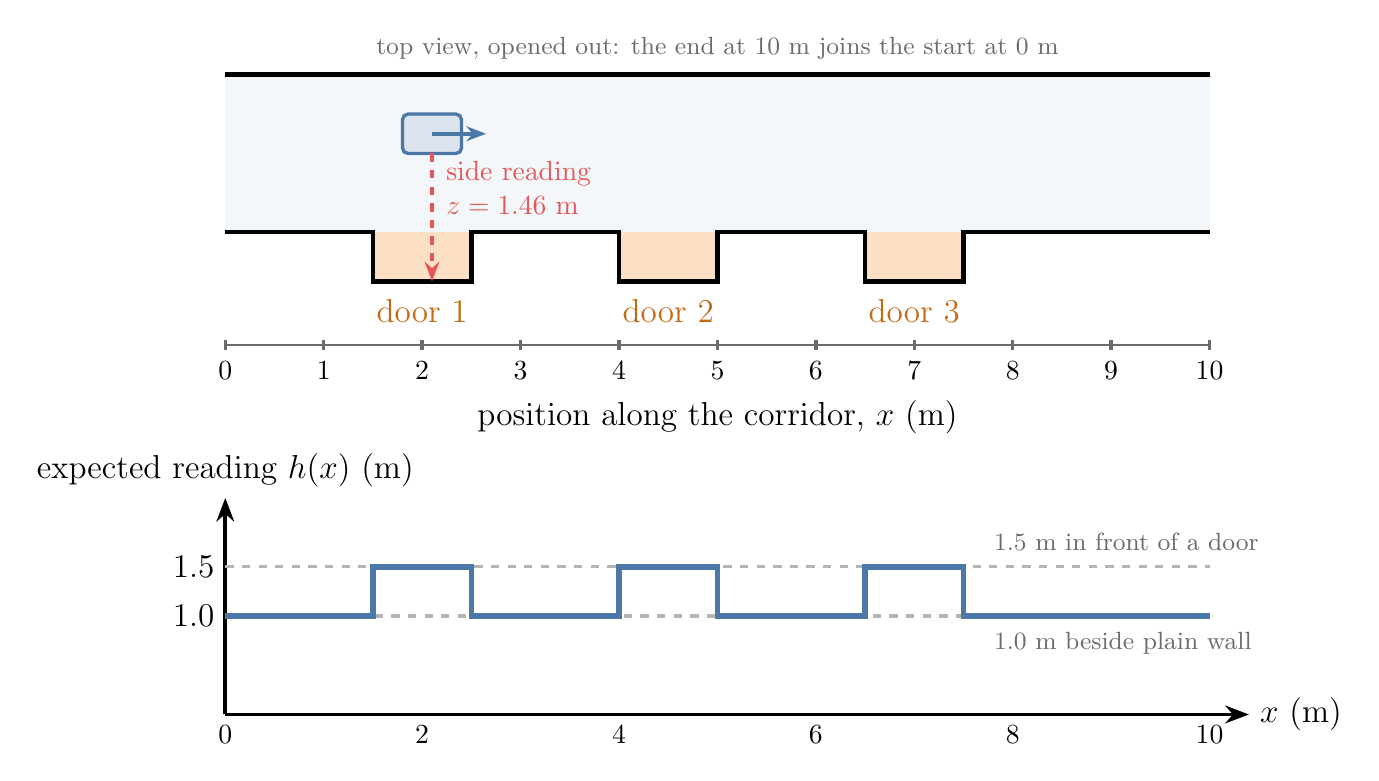
\begin{tikzpicture}[xscale=1.25, yscale=1.25, every node/.append style={font=\large}]
  % corridor floor (top view): left wall at y = 1.6, right wall at y = 0 with recesses down to y = -0.5
  \fill[cblue!6] (0,0) rectangle (10,1.6);
  \foreach \a/\b in {1.5/2.5, 4/5, 6.5/7.5} \fill[corange!25] (\a,-0.5) rectangle (\b,0);
  \draw[black, line width=1.6pt] (0,1.6) -- (10,1.6);
  \draw[black, line width=1.6pt] (0,0) -- (1.5,0) -- (1.5,-0.5) -- (2.5,-0.5) -- (2.5,0) -- (4,0) -- (4,-0.5) -- (5,-0.5)
        -- (5,0) -- (6.5,0) -- (6.5,-0.5) -- (7.5,-0.5) -- (7.5,0) -- (10,0);
  \node[corange!80!black] at (2,-0.8) {door 1};
  \node[corange!80!black] at (4.5,-0.8) {door 2};
  \node[corange!80!black] at (7,-0.8) {door 3};
  % robot at x = 2.1, centre line y = 1.0 (1.0 m from the right wall line), facing +x
  \begin{scope}[shift={(2.1,1.0)}]
    \draw[cblue, fill=cblue!20, rounded corners=2pt] (-0.3,-0.2) rectangle (0.3,0.2);
    \draw[-{Stealth[length=2.5mm]}, cblue, line width=1.6pt] (0,0) -- (0.55,0);
  \end{scope}
  \draw[cred, dashed, line width=1.4pt, -{Stealth[length=2.5mm]}] (2.1,0.8) -- (2.1,-0.5);
  \node[cred, right, align=left, font=\normalsize, fill=cblue!6, inner sep=1pt] at (2.2,0.45) {side reading\\$z = 1.46$ m};
  \node[note, anchor=south] at (5,1.65) {top view, opened out: the end at 10 m joins the start at 0 m};
  % axis
  \draw[cgrey, line width=0.8pt] (0,-1.15) -- (10,-1.15);
  \foreach \i in {0,...,10} {\draw[cgrey] (\i,-1.1) -- (\i,-1.2); \node[below, font=\normalsize] at (\i,-1.2) {\i};}
  \node[below] at (5,-1.6) {position along the corridor, $x$ (m)};
  % the map h(x)
  \begin{scope}[shift={(0,-4.9)}]
    \draw[arrow, draw=black] (0,0) -- (10.4,0) node[right] {$x$ (m)};
    \draw[arrow, draw=black] (0,0) -- (0,2.2) node[above, align=center] {expected reading $h(x)$ (m)};
    \draw[cgrey!50, dashed] (0,1) -- (10,1);
    \draw[cgrey!50, dashed] (0,1.5) -- (10,1.5);
    \node[left] at (0,1) {1.0};
    \node[left] at (0,1.5) {1.5};
    \draw[cblue, line width=2pt] (0,1) -- (1.5,1) -- (1.5,1.5) -- (2.5,1.5) -- (2.5,1) -- (4,1) -- (4,1.5) -- (5,1.5)
         -- (5,1) -- (6.5,1) -- (6.5,1.5) -- (7.5,1.5) -- (7.5,1) -- (10,1);
    \foreach \i in {0,2,...,10} \node[below, font=\normalsize] at (\i,0) {\i};
    \node[note, anchor=west] at (7.7,1.75) {1.5 m in front of a door};
    \node[note, anchor=west] at (7.7,0.72) {1.0 m beside plain wall};
  \end{scope}
\end{tikzpicture}
\end{document}
